% Created by tikzDevice version 0.12 on 2019-04-11 07:16:06
% !TEX encoding = UTF-8 Unicode
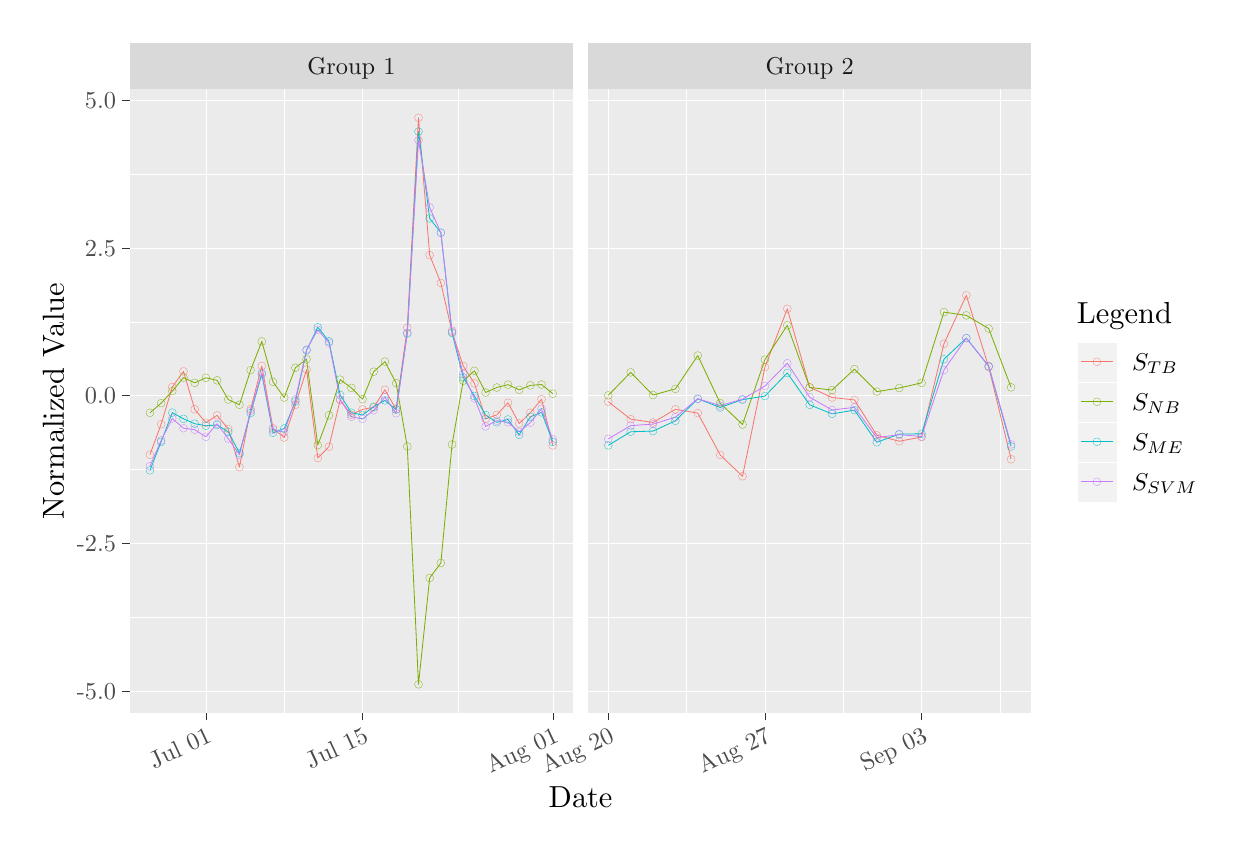
\begin{tikzpicture}[x=1pt,y=1pt]
\definecolor{fillColor}{RGB}{255,255,255}
\path[use as bounding box,fill=fillColor,fill opacity=0.00] (0,0) rectangle (433.62,289.08);
\begin{scope}
\path[clip] (  0.00,  0.00) rectangle (433.62,289.08);
\definecolor{drawColor}{RGB}{255,255,255}
\definecolor{fillColor}{RGB}{255,255,255}

\path[draw=drawColor,line width= 0.1pt,line join=round,line cap=round,fill=fillColor] (  0.00,  0.00) rectangle (433.62,289.08);
\end{scope}
\begin{scope}
\path[clip] ( 36.90, 41.55) rectangle (197.01,266.77);
\definecolor{fillColor}{gray}{0.92}

\path[fill=fillColor] ( 36.90, 41.55) rectangle (197.01,266.77);
\definecolor{drawColor}{RGB}{255,255,255}

\path[draw=drawColor,line width= 0.1pt,line join=round] ( 36.90, 76.16) --
	(197.01, 76.16);

\path[draw=drawColor,line width= 0.1pt,line join=round] ( 36.90,129.49) --
	(197.01,129.49);

\path[draw=drawColor,line width= 0.1pt,line join=round] ( 36.90,182.82) --
	(197.01,182.82);

\path[draw=drawColor,line width= 0.1pt,line join=round] ( 36.90,236.15) --
	(197.01,236.15);

\path[draw=drawColor,line width= 0.1pt,line join=round] ( 92.70, 41.55) --
	( 92.70,266.77);

\path[draw=drawColor,line width= 0.1pt,line join=round] (155.37, 41.55) --
	(155.37,266.77);

\path[draw=drawColor,line width= 0.1pt,line join=round] ( 36.90, 49.49) --
	(197.01, 49.49);

\path[draw=drawColor,line width= 0.1pt,line join=round] ( 36.90,102.82) --
	(197.01,102.82);

\path[draw=drawColor,line width= 0.1pt,line join=round] ( 36.90,156.15) --
	(197.01,156.15);

\path[draw=drawColor,line width= 0.1pt,line join=round] ( 36.90,209.49) --
	(197.01,209.49);

\path[draw=drawColor,line width= 0.1pt,line join=round] ( 36.90,262.82) --
	(197.01,262.82);

\path[draw=drawColor,line width= 0.1pt,line join=round] ( 64.39, 41.55) --
	( 64.39,266.77);

\path[draw=drawColor,line width= 0.1pt,line join=round] (121.00, 41.55) --
	(121.00,266.77);

\path[draw=drawColor,line width= 0.1pt,line join=round] (189.74, 41.55) --
	(189.74,266.77);
\definecolor{drawColor}{RGB}{248,118,109}

\path[draw=drawColor,line width= 0.3pt,line join=round] ( 44.18,134.77) --
	( 48.22,145.78) --
	( 52.26,159.24) --
	( 56.31,164.89) --
	( 60.35,151.18) --
	( 64.39,146.32) --
	( 68.44,148.99) --
	( 72.48,144.09) --
	( 76.52,130.30) --
	( 80.57,151.26) --
	( 84.61,166.85) --
	( 88.65,144.30) --
	( 92.70,140.95) --
	( 96.74,152.78) --
	(100.78,165.52) --
	(104.83,133.58) --
	(108.87,137.67) --
	(112.91,154.52) --
	(116.96,149.23) --
	(121.00,151.14) --
	(125.04,151.87) --
	(129.09,158.22) --
	(133.13,151.20) --
	(137.17,180.67) --
	(141.22,256.54) --
	(145.26,206.89) --
	(149.30,196.82) --
	(153.35,179.12) --
	(157.39,166.84) --
	(161.43,160.56) --
	(165.48,147.76) --
	(169.52,149.17) --
	(173.56,153.54) --
	(177.61,146.04) --
	(181.65,149.96) --
	(185.69,154.82) --
	(189.74,138.13);
\definecolor{drawColor}{RGB}{124,174,0}

\path[draw=drawColor,line width= 0.3pt,line join=round] ( 44.18,149.90) --
	( 48.22,153.40) --
	( 52.26,157.75) --
	( 56.31,162.64) --
	( 60.35,160.74) --
	( 64.39,162.56) --
	( 68.44,161.65) --
	( 72.48,154.70) --
	( 76.52,152.81) --
	( 80.57,165.32) --
	( 84.61,175.71) --
	( 88.65,161.10) --
	( 92.70,155.43) --
	( 96.74,166.19) --
	(100.78,169.27) --
	(104.83,138.23) --
	(108.87,149.02) --
	(112.91,161.90) --
	(116.96,158.93) --
	(121.00,154.83) --
	(125.04,164.76) --
	(129.09,168.42) --
	(133.13,160.68) --
	(137.17,137.76) --
	(141.22, 51.79) --
	(145.26, 90.22) --
	(149.30, 95.64) --
	(153.35,138.46) --
	(157.39,161.52) --
	(161.43,165.09) --
	(165.48,157.26) --
	(169.52,159.06) --
	(173.56,160.09) --
	(177.61,158.21) --
	(181.65,159.83) --
	(185.69,160.13) --
	(189.74,156.82);
\definecolor{drawColor}{RGB}{0,191,196}

\path[draw=drawColor,line width= 0.3pt,line join=round] ( 44.18,129.12) --
	( 48.22,139.41) --
	( 52.26,149.98) --
	( 56.31,147.73) --
	( 60.35,145.97) --
	( 64.39,145.24) --
	( 68.44,145.51) --
	( 72.48,143.05) --
	( 76.52,135.37) --
	( 80.57,149.86) --
	( 84.61,163.87) --
	( 88.65,142.69) --
	( 92.70,144.24) --
	( 96.74,153.99) --
	(100.78,172.48) --
	(104.83,180.84) --
	(108.87,175.76) --
	(112.91,156.35) --
	(116.96,149.96) --
	(121.00,149.12) --
	(125.04,152.12) --
	(129.09,154.40) --
	(133.13,151.06) --
	(137.17,178.52) --
	(141.22,251.54) --
	(145.26,220.15) --
	(149.30,215.00) --
	(153.35,178.75) --
	(157.39,162.70) --
	(161.43,155.98) --
	(165.48,149.09) --
	(169.52,146.46) --
	(173.56,147.51) --
	(177.61,141.93) --
	(181.65,148.47) --
	(185.69,150.07) --
	(189.74,139.40);
\definecolor{drawColor}{RGB}{199,124,255}

\path[draw=drawColor,line width= 0.3pt,line join=round] ( 44.18,130.58) --
	( 48.22,139.92) --
	( 52.26,147.88) --
	( 56.31,144.35) --
	( 60.35,143.81) --
	( 64.39,141.24) --
	( 68.44,145.94) --
	( 72.48,140.59) --
	( 76.52,134.74) --
	( 80.57,150.62) --
	( 84.61,164.43) --
	( 88.65,143.71) --
	( 92.70,142.87) --
	( 96.74,154.74) --
	(100.78,172.75) --
	(104.83,179.91) --
	(108.87,175.20) --
	(112.91,154.69) --
	(116.96,148.49) --
	(121.00,147.70) --
	(125.04,150.83) --
	(129.09,155.57) --
	(133.13,149.76) --
	(137.17,178.84) --
	(141.22,248.39) --
	(145.26,224.13) --
	(149.30,214.96) --
	(153.35,179.59) --
	(157.39,163.91) --
	(161.43,155.12) --
	(165.48,145.00) --
	(169.52,147.06) --
	(173.56,146.48) --
	(177.61,143.03) --
	(181.65,146.38) --
	(185.69,151.33) --
	(189.74,140.28);
\definecolor{drawColor}{RGB}{248,118,109}

\path[draw=drawColor,line width= 0.1pt,line join=round,line cap=round] ( 44.18,134.77) circle (  1.43);

\path[draw=drawColor,line width= 0.1pt,line join=round,line cap=round] ( 48.22,145.78) circle (  1.43);

\path[draw=drawColor,line width= 0.1pt,line join=round,line cap=round] ( 52.26,159.24) circle (  1.43);

\path[draw=drawColor,line width= 0.1pt,line join=round,line cap=round] ( 56.31,164.89) circle (  1.43);

\path[draw=drawColor,line width= 0.1pt,line join=round,line cap=round] ( 60.35,151.18) circle (  1.43);

\path[draw=drawColor,line width= 0.1pt,line join=round,line cap=round] ( 64.39,146.32) circle (  1.43);

\path[draw=drawColor,line width= 0.1pt,line join=round,line cap=round] ( 68.44,148.99) circle (  1.43);

\path[draw=drawColor,line width= 0.1pt,line join=round,line cap=round] ( 72.48,144.09) circle (  1.43);

\path[draw=drawColor,line width= 0.1pt,line join=round,line cap=round] ( 76.52,130.30) circle (  1.43);

\path[draw=drawColor,line width= 0.1pt,line join=round,line cap=round] ( 80.57,151.26) circle (  1.43);

\path[draw=drawColor,line width= 0.1pt,line join=round,line cap=round] ( 84.61,166.85) circle (  1.43);

\path[draw=drawColor,line width= 0.1pt,line join=round,line cap=round] ( 88.65,144.30) circle (  1.43);

\path[draw=drawColor,line width= 0.1pt,line join=round,line cap=round] ( 92.70,140.95) circle (  1.43);

\path[draw=drawColor,line width= 0.1pt,line join=round,line cap=round] ( 96.74,152.78) circle (  1.43);

\path[draw=drawColor,line width= 0.1pt,line join=round,line cap=round] (100.78,165.52) circle (  1.43);

\path[draw=drawColor,line width= 0.1pt,line join=round,line cap=round] (104.83,133.58) circle (  1.43);

\path[draw=drawColor,line width= 0.1pt,line join=round,line cap=round] (108.87,137.67) circle (  1.43);

\path[draw=drawColor,line width= 0.1pt,line join=round,line cap=round] (112.91,154.52) circle (  1.43);

\path[draw=drawColor,line width= 0.1pt,line join=round,line cap=round] (116.96,149.23) circle (  1.43);

\path[draw=drawColor,line width= 0.1pt,line join=round,line cap=round] (121.00,151.14) circle (  1.43);

\path[draw=drawColor,line width= 0.1pt,line join=round,line cap=round] (125.04,151.87) circle (  1.43);

\path[draw=drawColor,line width= 0.1pt,line join=round,line cap=round] (129.09,158.22) circle (  1.43);

\path[draw=drawColor,line width= 0.1pt,line join=round,line cap=round] (133.13,151.20) circle (  1.43);

\path[draw=drawColor,line width= 0.1pt,line join=round,line cap=round] (137.17,180.67) circle (  1.43);

\path[draw=drawColor,line width= 0.1pt,line join=round,line cap=round] (141.22,256.54) circle (  1.43);

\path[draw=drawColor,line width= 0.1pt,line join=round,line cap=round] (145.26,206.89) circle (  1.43);

\path[draw=drawColor,line width= 0.1pt,line join=round,line cap=round] (149.30,196.82) circle (  1.43);

\path[draw=drawColor,line width= 0.1pt,line join=round,line cap=round] (153.35,179.12) circle (  1.43);

\path[draw=drawColor,line width= 0.1pt,line join=round,line cap=round] (157.39,166.84) circle (  1.43);

\path[draw=drawColor,line width= 0.1pt,line join=round,line cap=round] (161.43,160.56) circle (  1.43);

\path[draw=drawColor,line width= 0.1pt,line join=round,line cap=round] (165.48,147.76) circle (  1.43);

\path[draw=drawColor,line width= 0.1pt,line join=round,line cap=round] (169.52,149.17) circle (  1.43);

\path[draw=drawColor,line width= 0.1pt,line join=round,line cap=round] (173.56,153.54) circle (  1.43);

\path[draw=drawColor,line width= 0.1pt,line join=round,line cap=round] (177.61,146.04) circle (  1.43);

\path[draw=drawColor,line width= 0.1pt,line join=round,line cap=round] (181.65,149.96) circle (  1.43);

\path[draw=drawColor,line width= 0.1pt,line join=round,line cap=round] (185.69,154.82) circle (  1.43);

\path[draw=drawColor,line width= 0.1pt,line join=round,line cap=round] (189.74,138.13) circle (  1.43);
\definecolor{drawColor}{RGB}{124,174,0}

\path[draw=drawColor,line width= 0.1pt,line join=round,line cap=round] ( 44.18,149.90) circle (  1.43);

\path[draw=drawColor,line width= 0.1pt,line join=round,line cap=round] ( 48.22,153.40) circle (  1.43);

\path[draw=drawColor,line width= 0.1pt,line join=round,line cap=round] ( 52.26,157.75) circle (  1.43);

\path[draw=drawColor,line width= 0.1pt,line join=round,line cap=round] ( 56.31,162.64) circle (  1.43);

\path[draw=drawColor,line width= 0.1pt,line join=round,line cap=round] ( 60.35,160.74) circle (  1.43);

\path[draw=drawColor,line width= 0.1pt,line join=round,line cap=round] ( 64.39,162.56) circle (  1.43);

\path[draw=drawColor,line width= 0.1pt,line join=round,line cap=round] ( 68.44,161.65) circle (  1.43);

\path[draw=drawColor,line width= 0.1pt,line join=round,line cap=round] ( 72.48,154.70) circle (  1.43);

\path[draw=drawColor,line width= 0.1pt,line join=round,line cap=round] ( 76.52,152.81) circle (  1.43);

\path[draw=drawColor,line width= 0.1pt,line join=round,line cap=round] ( 80.57,165.32) circle (  1.43);

\path[draw=drawColor,line width= 0.1pt,line join=round,line cap=round] ( 84.61,175.71) circle (  1.43);

\path[draw=drawColor,line width= 0.1pt,line join=round,line cap=round] ( 88.65,161.10) circle (  1.43);

\path[draw=drawColor,line width= 0.1pt,line join=round,line cap=round] ( 92.70,155.43) circle (  1.43);

\path[draw=drawColor,line width= 0.1pt,line join=round,line cap=round] ( 96.74,166.19) circle (  1.43);

\path[draw=drawColor,line width= 0.1pt,line join=round,line cap=round] (100.78,169.27) circle (  1.43);

\path[draw=drawColor,line width= 0.1pt,line join=round,line cap=round] (104.83,138.23) circle (  1.43);

\path[draw=drawColor,line width= 0.1pt,line join=round,line cap=round] (108.87,149.02) circle (  1.43);

\path[draw=drawColor,line width= 0.1pt,line join=round,line cap=round] (112.91,161.90) circle (  1.43);

\path[draw=drawColor,line width= 0.1pt,line join=round,line cap=round] (116.96,158.93) circle (  1.43);

\path[draw=drawColor,line width= 0.1pt,line join=round,line cap=round] (121.00,154.83) circle (  1.43);

\path[draw=drawColor,line width= 0.1pt,line join=round,line cap=round] (125.04,164.76) circle (  1.43);

\path[draw=drawColor,line width= 0.1pt,line join=round,line cap=round] (129.09,168.42) circle (  1.43);

\path[draw=drawColor,line width= 0.1pt,line join=round,line cap=round] (133.13,160.68) circle (  1.43);

\path[draw=drawColor,line width= 0.1pt,line join=round,line cap=round] (137.17,137.76) circle (  1.43);

\path[draw=drawColor,line width= 0.1pt,line join=round,line cap=round] (141.22, 51.79) circle (  1.43);

\path[draw=drawColor,line width= 0.1pt,line join=round,line cap=round] (145.26, 90.22) circle (  1.43);

\path[draw=drawColor,line width= 0.1pt,line join=round,line cap=round] (149.30, 95.64) circle (  1.43);

\path[draw=drawColor,line width= 0.1pt,line join=round,line cap=round] (153.35,138.46) circle (  1.43);

\path[draw=drawColor,line width= 0.1pt,line join=round,line cap=round] (157.39,161.52) circle (  1.43);

\path[draw=drawColor,line width= 0.1pt,line join=round,line cap=round] (161.43,165.09) circle (  1.43);

\path[draw=drawColor,line width= 0.1pt,line join=round,line cap=round] (165.48,157.26) circle (  1.43);

\path[draw=drawColor,line width= 0.1pt,line join=round,line cap=round] (169.52,159.06) circle (  1.43);

\path[draw=drawColor,line width= 0.1pt,line join=round,line cap=round] (173.56,160.09) circle (  1.43);

\path[draw=drawColor,line width= 0.1pt,line join=round,line cap=round] (177.61,158.21) circle (  1.43);

\path[draw=drawColor,line width= 0.1pt,line join=round,line cap=round] (181.65,159.83) circle (  1.43);

\path[draw=drawColor,line width= 0.1pt,line join=round,line cap=round] (185.69,160.13) circle (  1.43);

\path[draw=drawColor,line width= 0.1pt,line join=round,line cap=round] (189.74,156.82) circle (  1.43);
\definecolor{drawColor}{RGB}{0,191,196}

\path[draw=drawColor,line width= 0.1pt,line join=round,line cap=round] ( 44.18,129.12) circle (  1.43);

\path[draw=drawColor,line width= 0.1pt,line join=round,line cap=round] ( 48.22,139.41) circle (  1.43);

\path[draw=drawColor,line width= 0.1pt,line join=round,line cap=round] ( 52.26,149.98) circle (  1.43);

\path[draw=drawColor,line width= 0.1pt,line join=round,line cap=round] ( 56.31,147.73) circle (  1.43);

\path[draw=drawColor,line width= 0.1pt,line join=round,line cap=round] ( 60.35,145.97) circle (  1.43);

\path[draw=drawColor,line width= 0.1pt,line join=round,line cap=round] ( 64.39,145.24) circle (  1.43);

\path[draw=drawColor,line width= 0.1pt,line join=round,line cap=round] ( 68.44,145.51) circle (  1.43);

\path[draw=drawColor,line width= 0.1pt,line join=round,line cap=round] ( 72.48,143.05) circle (  1.43);

\path[draw=drawColor,line width= 0.1pt,line join=round,line cap=round] ( 76.52,135.37) circle (  1.43);

\path[draw=drawColor,line width= 0.1pt,line join=round,line cap=round] ( 80.57,149.86) circle (  1.43);

\path[draw=drawColor,line width= 0.1pt,line join=round,line cap=round] ( 84.61,163.87) circle (  1.43);

\path[draw=drawColor,line width= 0.1pt,line join=round,line cap=round] ( 88.65,142.69) circle (  1.43);

\path[draw=drawColor,line width= 0.1pt,line join=round,line cap=round] ( 92.70,144.24) circle (  1.43);

\path[draw=drawColor,line width= 0.1pt,line join=round,line cap=round] ( 96.74,153.99) circle (  1.43);

\path[draw=drawColor,line width= 0.1pt,line join=round,line cap=round] (100.78,172.48) circle (  1.43);

\path[draw=drawColor,line width= 0.1pt,line join=round,line cap=round] (104.83,180.84) circle (  1.43);

\path[draw=drawColor,line width= 0.1pt,line join=round,line cap=round] (108.87,175.76) circle (  1.43);

\path[draw=drawColor,line width= 0.1pt,line join=round,line cap=round] (112.91,156.35) circle (  1.43);

\path[draw=drawColor,line width= 0.1pt,line join=round,line cap=round] (116.96,149.96) circle (  1.43);

\path[draw=drawColor,line width= 0.1pt,line join=round,line cap=round] (121.00,149.12) circle (  1.43);

\path[draw=drawColor,line width= 0.1pt,line join=round,line cap=round] (125.04,152.12) circle (  1.43);

\path[draw=drawColor,line width= 0.1pt,line join=round,line cap=round] (129.09,154.40) circle (  1.43);

\path[draw=drawColor,line width= 0.1pt,line join=round,line cap=round] (133.13,151.06) circle (  1.43);

\path[draw=drawColor,line width= 0.1pt,line join=round,line cap=round] (137.17,178.52) circle (  1.43);

\path[draw=drawColor,line width= 0.1pt,line join=round,line cap=round] (141.22,251.54) circle (  1.43);

\path[draw=drawColor,line width= 0.1pt,line join=round,line cap=round] (145.26,220.15) circle (  1.43);

\path[draw=drawColor,line width= 0.1pt,line join=round,line cap=round] (149.30,215.00) circle (  1.43);

\path[draw=drawColor,line width= 0.1pt,line join=round,line cap=round] (153.35,178.75) circle (  1.43);

\path[draw=drawColor,line width= 0.1pt,line join=round,line cap=round] (157.39,162.70) circle (  1.43);

\path[draw=drawColor,line width= 0.1pt,line join=round,line cap=round] (161.43,155.98) circle (  1.43);

\path[draw=drawColor,line width= 0.1pt,line join=round,line cap=round] (165.48,149.09) circle (  1.43);

\path[draw=drawColor,line width= 0.1pt,line join=round,line cap=round] (169.52,146.46) circle (  1.43);

\path[draw=drawColor,line width= 0.1pt,line join=round,line cap=round] (173.56,147.51) circle (  1.43);

\path[draw=drawColor,line width= 0.1pt,line join=round,line cap=round] (177.61,141.93) circle (  1.43);

\path[draw=drawColor,line width= 0.1pt,line join=round,line cap=round] (181.65,148.47) circle (  1.43);

\path[draw=drawColor,line width= 0.1pt,line join=round,line cap=round] (185.69,150.07) circle (  1.43);

\path[draw=drawColor,line width= 0.1pt,line join=round,line cap=round] (189.74,139.40) circle (  1.43);
\definecolor{drawColor}{RGB}{199,124,255}

\path[draw=drawColor,line width= 0.1pt,line join=round,line cap=round] ( 44.18,130.58) circle (  1.43);

\path[draw=drawColor,line width= 0.1pt,line join=round,line cap=round] ( 48.22,139.92) circle (  1.43);

\path[draw=drawColor,line width= 0.1pt,line join=round,line cap=round] ( 52.26,147.88) circle (  1.43);

\path[draw=drawColor,line width= 0.1pt,line join=round,line cap=round] ( 56.31,144.35) circle (  1.43);

\path[draw=drawColor,line width= 0.1pt,line join=round,line cap=round] ( 60.35,143.81) circle (  1.43);

\path[draw=drawColor,line width= 0.1pt,line join=round,line cap=round] ( 64.39,141.24) circle (  1.43);

\path[draw=drawColor,line width= 0.1pt,line join=round,line cap=round] ( 68.44,145.94) circle (  1.43);

\path[draw=drawColor,line width= 0.1pt,line join=round,line cap=round] ( 72.48,140.59) circle (  1.43);

\path[draw=drawColor,line width= 0.1pt,line join=round,line cap=round] ( 76.52,134.74) circle (  1.43);

\path[draw=drawColor,line width= 0.1pt,line join=round,line cap=round] ( 80.57,150.62) circle (  1.43);

\path[draw=drawColor,line width= 0.1pt,line join=round,line cap=round] ( 84.61,164.43) circle (  1.43);

\path[draw=drawColor,line width= 0.1pt,line join=round,line cap=round] ( 88.65,143.71) circle (  1.43);

\path[draw=drawColor,line width= 0.1pt,line join=round,line cap=round] ( 92.70,142.87) circle (  1.43);

\path[draw=drawColor,line width= 0.1pt,line join=round,line cap=round] ( 96.74,154.74) circle (  1.43);

\path[draw=drawColor,line width= 0.1pt,line join=round,line cap=round] (100.78,172.75) circle (  1.43);

\path[draw=drawColor,line width= 0.1pt,line join=round,line cap=round] (104.83,179.91) circle (  1.43);

\path[draw=drawColor,line width= 0.1pt,line join=round,line cap=round] (108.87,175.20) circle (  1.43);

\path[draw=drawColor,line width= 0.1pt,line join=round,line cap=round] (112.91,154.69) circle (  1.43);

\path[draw=drawColor,line width= 0.1pt,line join=round,line cap=round] (116.96,148.49) circle (  1.43);

\path[draw=drawColor,line width= 0.1pt,line join=round,line cap=round] (121.00,147.70) circle (  1.43);

\path[draw=drawColor,line width= 0.1pt,line join=round,line cap=round] (125.04,150.83) circle (  1.43);

\path[draw=drawColor,line width= 0.1pt,line join=round,line cap=round] (129.09,155.57) circle (  1.43);

\path[draw=drawColor,line width= 0.1pt,line join=round,line cap=round] (133.13,149.76) circle (  1.43);

\path[draw=drawColor,line width= 0.1pt,line join=round,line cap=round] (137.17,178.84) circle (  1.43);

\path[draw=drawColor,line width= 0.1pt,line join=round,line cap=round] (141.22,248.39) circle (  1.43);

\path[draw=drawColor,line width= 0.1pt,line join=round,line cap=round] (145.26,224.13) circle (  1.43);

\path[draw=drawColor,line width= 0.1pt,line join=round,line cap=round] (149.30,214.96) circle (  1.43);

\path[draw=drawColor,line width= 0.1pt,line join=round,line cap=round] (153.35,179.59) circle (  1.43);

\path[draw=drawColor,line width= 0.1pt,line join=round,line cap=round] (157.39,163.91) circle (  1.43);

\path[draw=drawColor,line width= 0.1pt,line join=round,line cap=round] (161.43,155.12) circle (  1.43);

\path[draw=drawColor,line width= 0.1pt,line join=round,line cap=round] (165.48,145.00) circle (  1.43);

\path[draw=drawColor,line width= 0.1pt,line join=round,line cap=round] (169.52,147.06) circle (  1.43);

\path[draw=drawColor,line width= 0.1pt,line join=round,line cap=round] (173.56,146.48) circle (  1.43);

\path[draw=drawColor,line width= 0.1pt,line join=round,line cap=round] (177.61,143.03) circle (  1.43);

\path[draw=drawColor,line width= 0.1pt,line join=round,line cap=round] (181.65,146.38) circle (  1.43);

\path[draw=drawColor,line width= 0.1pt,line join=round,line cap=round] (185.69,151.33) circle (  1.43);

\path[draw=drawColor,line width= 0.1pt,line join=round,line cap=round] (189.74,140.28) circle (  1.43);
\end{scope}
\begin{scope}
\path[clip] (202.51, 41.55) rectangle (362.63,266.77);
\definecolor{fillColor}{gray}{0.92}

\path[fill=fillColor] (202.51, 41.55) rectangle (362.63,266.77);
\definecolor{drawColor}{RGB}{255,255,255}

\path[draw=drawColor,line width= 0.1pt,line join=round] (202.51, 76.16) --
	(362.63, 76.16);

\path[draw=drawColor,line width= 0.1pt,line join=round] (202.51,129.49) --
	(362.63,129.49);

\path[draw=drawColor,line width= 0.1pt,line join=round] (202.51,182.82) --
	(362.63,182.82);

\path[draw=drawColor,line width= 0.1pt,line join=round] (202.51,236.15) --
	(362.63,236.15);

\path[draw=drawColor,line width= 0.1pt,line join=round] (238.10, 41.55) --
	(238.10,266.77);

\path[draw=drawColor,line width= 0.1pt,line join=round] (294.70, 41.55) --
	(294.70,266.77);

\path[draw=drawColor,line width= 0.1pt,line join=round] (351.31, 41.55) --
	(351.31,266.77);

\path[draw=drawColor,line width= 0.1pt,line join=round] (202.51, 49.49) --
	(362.63, 49.49);

\path[draw=drawColor,line width= 0.1pt,line join=round] (202.51,102.82) --
	(362.63,102.82);

\path[draw=drawColor,line width= 0.1pt,line join=round] (202.51,156.15) --
	(362.63,156.15);

\path[draw=drawColor,line width= 0.1pt,line join=round] (202.51,209.49) --
	(362.63,209.49);

\path[draw=drawColor,line width= 0.1pt,line join=round] (202.51,262.82) --
	(362.63,262.82);

\path[draw=drawColor,line width= 0.1pt,line join=round] (209.79, 41.55) --
	(209.79,266.77);

\path[draw=drawColor,line width= 0.1pt,line join=round] (266.40, 41.55) --
	(266.40,266.77);

\path[draw=drawColor,line width= 0.1pt,line join=round] (323.01, 41.55) --
	(323.01,266.77);
\definecolor{drawColor}{RGB}{248,118,109}

\path[draw=drawColor,line width= 0.3pt,line join=round] (209.79,153.95) --
	(217.88,147.62) --
	(225.97,146.40) --
	(234.05,151.17) --
	(242.14,149.81) --
	(250.23,134.71) --
	(258.31,126.98) --
	(266.40,166.43) --
	(274.49,187.49) --
	(282.57,159.14) --
	(290.66,155.43) --
	(298.75,154.57) --
	(306.83,141.79) --
	(314.92,139.63) --
	(323.01,141.16) --
	(331.09,174.87) --
	(339.18,192.34) --
	(347.26,166.49) --
	(355.35,133.14);
\definecolor{drawColor}{RGB}{124,174,0}

\path[draw=drawColor,line width= 0.3pt,line join=round] (209.79,156.21) --
	(217.88,164.52) --
	(225.97,156.32) --
	(234.05,158.57) --
	(242.14,170.59) --
	(250.23,153.40) --
	(258.31,145.69) --
	(266.40,169.10) --
	(274.49,181.52) --
	(282.57,159.09) --
	(290.66,158.12) --
	(298.75,165.70) --
	(306.83,157.56) --
	(314.92,158.87) --
	(323.01,160.73) --
	(331.09,186.30) --
	(339.18,185.11) --
	(347.26,180.34) --
	(355.35,159.12);
\definecolor{drawColor}{RGB}{0,191,196}

\path[draw=drawColor,line width= 0.3pt,line join=round] (209.79,138.14) --
	(217.88,143.06) --
	(225.97,143.30) --
	(234.05,147.02) --
	(242.14,154.97) --
	(250.23,151.84) --
	(258.31,154.67) --
	(266.40,155.96) --
	(274.49,164.29) --
	(282.57,152.78) --
	(290.66,149.54) --
	(298.75,150.89) --
	(306.83,139.26) --
	(314.92,142.23) --
	(323.01,142.31) --
	(331.09,169.26) --
	(339.18,176.92) --
	(347.26,166.75) --
	(355.35,137.75);
\definecolor{drawColor}{RGB}{199,124,255}

\path[draw=drawColor,line width= 0.3pt,line join=round] (209.79,140.46) --
	(217.88,145.28) --
	(225.97,145.83) --
	(234.05,148.31) --
	(242.14,154.98) --
	(250.23,152.51) --
	(258.31,154.83) --
	(266.40,159.58) --
	(274.49,167.82) --
	(282.57,155.55) --
	(290.66,150.92) --
	(298.75,151.87) --
	(306.83,140.93) --
	(314.92,142.02) --
	(323.01,141.35) --
	(331.09,165.37) --
	(339.18,176.90) --
	(347.26,166.80) --
	(355.35,138.51);
\definecolor{drawColor}{RGB}{248,118,109}

\path[draw=drawColor,line width= 0.1pt,line join=round,line cap=round] (209.79,153.95) circle (  1.43);

\path[draw=drawColor,line width= 0.1pt,line join=round,line cap=round] (217.88,147.62) circle (  1.43);

\path[draw=drawColor,line width= 0.1pt,line join=round,line cap=round] (225.97,146.40) circle (  1.43);

\path[draw=drawColor,line width= 0.1pt,line join=round,line cap=round] (234.05,151.17) circle (  1.43);

\path[draw=drawColor,line width= 0.1pt,line join=round,line cap=round] (242.14,149.81) circle (  1.43);

\path[draw=drawColor,line width= 0.1pt,line join=round,line cap=round] (250.23,134.71) circle (  1.43);

\path[draw=drawColor,line width= 0.1pt,line join=round,line cap=round] (258.31,126.98) circle (  1.43);

\path[draw=drawColor,line width= 0.1pt,line join=round,line cap=round] (266.40,166.43) circle (  1.43);

\path[draw=drawColor,line width= 0.1pt,line join=round,line cap=round] (274.49,187.49) circle (  1.43);

\path[draw=drawColor,line width= 0.1pt,line join=round,line cap=round] (282.57,159.14) circle (  1.43);

\path[draw=drawColor,line width= 0.1pt,line join=round,line cap=round] (290.66,155.43) circle (  1.43);

\path[draw=drawColor,line width= 0.1pt,line join=round,line cap=round] (298.75,154.57) circle (  1.43);

\path[draw=drawColor,line width= 0.1pt,line join=round,line cap=round] (306.83,141.79) circle (  1.43);

\path[draw=drawColor,line width= 0.1pt,line join=round,line cap=round] (314.92,139.63) circle (  1.43);

\path[draw=drawColor,line width= 0.1pt,line join=round,line cap=round] (323.01,141.16) circle (  1.43);

\path[draw=drawColor,line width= 0.1pt,line join=round,line cap=round] (331.09,174.87) circle (  1.43);

\path[draw=drawColor,line width= 0.1pt,line join=round,line cap=round] (339.18,192.34) circle (  1.43);

\path[draw=drawColor,line width= 0.1pt,line join=round,line cap=round] (347.26,166.49) circle (  1.43);

\path[draw=drawColor,line width= 0.1pt,line join=round,line cap=round] (355.35,133.14) circle (  1.43);
\definecolor{drawColor}{RGB}{124,174,0}

\path[draw=drawColor,line width= 0.1pt,line join=round,line cap=round] (209.79,156.21) circle (  1.43);

\path[draw=drawColor,line width= 0.1pt,line join=round,line cap=round] (217.88,164.52) circle (  1.43);

\path[draw=drawColor,line width= 0.1pt,line join=round,line cap=round] (225.97,156.32) circle (  1.43);

\path[draw=drawColor,line width= 0.1pt,line join=round,line cap=round] (234.05,158.57) circle (  1.43);

\path[draw=drawColor,line width= 0.1pt,line join=round,line cap=round] (242.14,170.59) circle (  1.43);

\path[draw=drawColor,line width= 0.1pt,line join=round,line cap=round] (250.23,153.40) circle (  1.43);

\path[draw=drawColor,line width= 0.1pt,line join=round,line cap=round] (258.31,145.69) circle (  1.43);

\path[draw=drawColor,line width= 0.1pt,line join=round,line cap=round] (266.40,169.10) circle (  1.43);

\path[draw=drawColor,line width= 0.1pt,line join=round,line cap=round] (274.49,181.52) circle (  1.43);

\path[draw=drawColor,line width= 0.1pt,line join=round,line cap=round] (282.57,159.09) circle (  1.43);

\path[draw=drawColor,line width= 0.1pt,line join=round,line cap=round] (290.66,158.12) circle (  1.43);

\path[draw=drawColor,line width= 0.1pt,line join=round,line cap=round] (298.75,165.70) circle (  1.43);

\path[draw=drawColor,line width= 0.1pt,line join=round,line cap=round] (306.83,157.56) circle (  1.43);

\path[draw=drawColor,line width= 0.1pt,line join=round,line cap=round] (314.92,158.87) circle (  1.43);

\path[draw=drawColor,line width= 0.1pt,line join=round,line cap=round] (323.01,160.73) circle (  1.43);

\path[draw=drawColor,line width= 0.1pt,line join=round,line cap=round] (331.09,186.30) circle (  1.43);

\path[draw=drawColor,line width= 0.1pt,line join=round,line cap=round] (339.18,185.11) circle (  1.43);

\path[draw=drawColor,line width= 0.1pt,line join=round,line cap=round] (347.26,180.34) circle (  1.43);

\path[draw=drawColor,line width= 0.1pt,line join=round,line cap=round] (355.35,159.12) circle (  1.43);
\definecolor{drawColor}{RGB}{0,191,196}

\path[draw=drawColor,line width= 0.1pt,line join=round,line cap=round] (209.79,138.14) circle (  1.43);

\path[draw=drawColor,line width= 0.1pt,line join=round,line cap=round] (217.88,143.06) circle (  1.43);

\path[draw=drawColor,line width= 0.1pt,line join=round,line cap=round] (225.97,143.30) circle (  1.43);

\path[draw=drawColor,line width= 0.1pt,line join=round,line cap=round] (234.05,147.02) circle (  1.43);

\path[draw=drawColor,line width= 0.1pt,line join=round,line cap=round] (242.14,154.97) circle (  1.43);

\path[draw=drawColor,line width= 0.1pt,line join=round,line cap=round] (250.23,151.84) circle (  1.43);

\path[draw=drawColor,line width= 0.1pt,line join=round,line cap=round] (258.31,154.67) circle (  1.43);

\path[draw=drawColor,line width= 0.1pt,line join=round,line cap=round] (266.40,155.96) circle (  1.43);

\path[draw=drawColor,line width= 0.1pt,line join=round,line cap=round] (274.49,164.29) circle (  1.43);

\path[draw=drawColor,line width= 0.1pt,line join=round,line cap=round] (282.57,152.78) circle (  1.43);

\path[draw=drawColor,line width= 0.1pt,line join=round,line cap=round] (290.66,149.54) circle (  1.43);

\path[draw=drawColor,line width= 0.1pt,line join=round,line cap=round] (298.75,150.89) circle (  1.43);

\path[draw=drawColor,line width= 0.1pt,line join=round,line cap=round] (306.83,139.26) circle (  1.43);

\path[draw=drawColor,line width= 0.1pt,line join=round,line cap=round] (314.92,142.23) circle (  1.43);

\path[draw=drawColor,line width= 0.1pt,line join=round,line cap=round] (323.01,142.31) circle (  1.43);

\path[draw=drawColor,line width= 0.1pt,line join=round,line cap=round] (331.09,169.26) circle (  1.43);

\path[draw=drawColor,line width= 0.1pt,line join=round,line cap=round] (339.18,176.92) circle (  1.43);

\path[draw=drawColor,line width= 0.1pt,line join=round,line cap=round] (347.26,166.75) circle (  1.43);

\path[draw=drawColor,line width= 0.1pt,line join=round,line cap=round] (355.35,137.75) circle (  1.43);
\definecolor{drawColor}{RGB}{199,124,255}

\path[draw=drawColor,line width= 0.1pt,line join=round,line cap=round] (209.79,140.46) circle (  1.43);

\path[draw=drawColor,line width= 0.1pt,line join=round,line cap=round] (217.88,145.28) circle (  1.43);

\path[draw=drawColor,line width= 0.1pt,line join=round,line cap=round] (225.97,145.83) circle (  1.43);

\path[draw=drawColor,line width= 0.1pt,line join=round,line cap=round] (234.05,148.31) circle (  1.43);

\path[draw=drawColor,line width= 0.1pt,line join=round,line cap=round] (242.14,154.98) circle (  1.43);

\path[draw=drawColor,line width= 0.1pt,line join=round,line cap=round] (250.23,152.51) circle (  1.43);

\path[draw=drawColor,line width= 0.1pt,line join=round,line cap=round] (258.31,154.83) circle (  1.43);

\path[draw=drawColor,line width= 0.1pt,line join=round,line cap=round] (266.40,159.58) circle (  1.43);

\path[draw=drawColor,line width= 0.1pt,line join=round,line cap=round] (274.49,167.82) circle (  1.43);

\path[draw=drawColor,line width= 0.1pt,line join=round,line cap=round] (282.57,155.55) circle (  1.43);

\path[draw=drawColor,line width= 0.1pt,line join=round,line cap=round] (290.66,150.92) circle (  1.43);

\path[draw=drawColor,line width= 0.1pt,line join=round,line cap=round] (298.75,151.87) circle (  1.43);

\path[draw=drawColor,line width= 0.1pt,line join=round,line cap=round] (306.83,140.93) circle (  1.43);

\path[draw=drawColor,line width= 0.1pt,line join=round,line cap=round] (314.92,142.02) circle (  1.43);

\path[draw=drawColor,line width= 0.1pt,line join=round,line cap=round] (323.01,141.35) circle (  1.43);

\path[draw=drawColor,line width= 0.1pt,line join=round,line cap=round] (331.09,165.37) circle (  1.43);

\path[draw=drawColor,line width= 0.1pt,line join=round,line cap=round] (339.18,176.90) circle (  1.43);

\path[draw=drawColor,line width= 0.1pt,line join=round,line cap=round] (347.26,166.80) circle (  1.43);

\path[draw=drawColor,line width= 0.1pt,line join=round,line cap=round] (355.35,138.51) circle (  1.43);
\end{scope}
\begin{scope}
\path[clip] ( 36.90,266.77) rectangle (197.01,283.58);
\definecolor{fillColor}{gray}{0.85}

\path[fill=fillColor] ( 36.90,266.77) rectangle (197.01,283.58);
\definecolor{drawColor}{gray}{0.10}

\node[text=drawColor,anchor=base,inner sep=0pt, outer sep=0pt, scale=  0.88] at (116.96,272.15) {Group 1};
\end{scope}
\begin{scope}
\path[clip] (202.51,266.77) rectangle (362.63,283.58);
\definecolor{fillColor}{gray}{0.85}

\path[fill=fillColor] (202.51,266.77) rectangle (362.63,283.58);
\definecolor{drawColor}{gray}{0.10}

\node[text=drawColor,anchor=base,inner sep=0pt, outer sep=0pt, scale=  0.88] at (282.57,272.15) {Group 2};
\end{scope}
\begin{scope}
\path[clip] (  0.00,  0.00) rectangle (433.62,289.08);
\definecolor{drawColor}{gray}{0.20}

\path[draw=drawColor,line width= 0.1pt,line join=round] ( 64.39, 38.80) --
	( 64.39, 41.55);

\path[draw=drawColor,line width= 0.1pt,line join=round] (121.00, 38.80) --
	(121.00, 41.55);

\path[draw=drawColor,line width= 0.1pt,line join=round] (189.74, 38.80) --
	(189.74, 41.55);
\end{scope}
\begin{scope}
\path[clip] (  0.00,  0.00) rectangle (433.62,289.08);
\definecolor{drawColor}{gray}{0.30}

\node[text=drawColor,rotate= 25.00,anchor=base east,inner sep=0pt, outer sep=0pt, scale=  0.88] at ( 66.96, 31.10) {Jul 01};

\node[text=drawColor,rotate= 25.00,anchor=base east,inner sep=0pt, outer sep=0pt, scale=  0.88] at (123.56, 31.10) {Jul 15};

\node[text=drawColor,rotate= 25.00,anchor=base east,inner sep=0pt, outer sep=0pt, scale=  0.88] at (192.30, 31.10) {Aug 01};
\end{scope}
\begin{scope}
\path[clip] (  0.00,  0.00) rectangle (433.62,289.08);
\definecolor{drawColor}{gray}{0.20}

\path[draw=drawColor,line width= 0.1pt,line join=round] (209.79, 38.80) --
	(209.79, 41.55);

\path[draw=drawColor,line width= 0.1pt,line join=round] (266.40, 38.80) --
	(266.40, 41.55);

\path[draw=drawColor,line width= 0.1pt,line join=round] (323.01, 38.80) --
	(323.01, 41.55);
\end{scope}
\begin{scope}
\path[clip] (  0.00,  0.00) rectangle (433.62,289.08);
\definecolor{drawColor}{gray}{0.30}

\node[text=drawColor,rotate= 25.00,anchor=base east,inner sep=0pt, outer sep=0pt, scale=  0.88] at (212.35, 31.10) {Aug 20};

\node[text=drawColor,rotate= 25.00,anchor=base east,inner sep=0pt, outer sep=0pt, scale=  0.88] at (268.96, 31.10) {Aug 27};

\node[text=drawColor,rotate= 25.00,anchor=base east,inner sep=0pt, outer sep=0pt, scale=  0.88] at (325.57, 31.10) {Sep 03};
\end{scope}
\begin{scope}
\path[clip] (  0.00,  0.00) rectangle (433.62,289.08);
\definecolor{drawColor}{gray}{0.30}

\node[text=drawColor,anchor=base east,inner sep=0pt, outer sep=0pt, scale=  0.88] at ( 31.95, 46.46) {-5.0};

\node[text=drawColor,anchor=base east,inner sep=0pt, outer sep=0pt, scale=  0.88] at ( 31.95, 99.79) {-2.5};

\node[text=drawColor,anchor=base east,inner sep=0pt, outer sep=0pt, scale=  0.88] at ( 31.95,153.12) {0.0};

\node[text=drawColor,anchor=base east,inner sep=0pt, outer sep=0pt, scale=  0.88] at ( 31.95,206.46) {2.5};

\node[text=drawColor,anchor=base east,inner sep=0pt, outer sep=0pt, scale=  0.88] at ( 31.95,259.79) {5.0};
\end{scope}
\begin{scope}
\path[clip] (  0.00,  0.00) rectangle (433.62,289.08);
\definecolor{drawColor}{gray}{0.20}

\path[draw=drawColor,line width= 0.1pt,line join=round] ( 34.15, 49.49) --
	( 36.90, 49.49);

\path[draw=drawColor,line width= 0.1pt,line join=round] ( 34.15,102.82) --
	( 36.90,102.82);

\path[draw=drawColor,line width= 0.1pt,line join=round] ( 34.15,156.15) --
	( 36.90,156.15);

\path[draw=drawColor,line width= 0.1pt,line join=round] ( 34.15,209.49) --
	( 36.90,209.49);

\path[draw=drawColor,line width= 0.1pt,line join=round] ( 34.15,262.82) --
	( 36.90,262.82);
\end{scope}
\begin{scope}
\path[clip] (  0.00,  0.00) rectangle (433.62,289.08);
\definecolor{drawColor}{RGB}{0,0,0}

\node[text=drawColor,anchor=base,inner sep=0pt, outer sep=0pt, scale=  1.10] at (199.76,  7.44) {Date};
\end{scope}
\begin{scope}
\path[clip] (  0.00,  0.00) rectangle (433.62,289.08);
\definecolor{drawColor}{RGB}{0,0,0}

\node[text=drawColor,rotate= 90.00,anchor=base,inner sep=0pt, outer sep=0pt, scale=  1.10] at ( 13.08,154.16) {Normalized Value};
\end{scope}
\begin{scope}
\path[clip] (  0.00,  0.00) rectangle (433.62,289.08);
\definecolor{fillColor}{RGB}{255,255,255}

\path[fill=fillColor] (373.63,112.24) rectangle (428.12,196.08);
\end{scope}
\begin{scope}
\path[clip] (  0.00,  0.00) rectangle (433.62,289.08);
\definecolor{drawColor}{RGB}{0,0,0}

\node[text=drawColor,anchor=base west,inner sep=0pt, outer sep=0pt, scale=  1.10] at (379.13,182.03) {Legend};
\end{scope}
\begin{scope}
\path[clip] (  0.00,  0.00) rectangle (433.62,289.08);
\definecolor{drawColor}{RGB}{255,255,255}
\definecolor{fillColor}{gray}{0.95}

\path[draw=drawColor,line width= 0.1pt,line join=round,line cap=round,fill=fillColor] (379.13,161.10) rectangle (393.58,175.56);
\end{scope}
\begin{scope}
\path[clip] (  0.00,  0.00) rectangle (433.62,289.08);
\definecolor{drawColor}{RGB}{248,118,109}

\path[draw=drawColor,line width= 0.3pt,line join=round] (380.57,168.33) -- (392.14,168.33);
\end{scope}
\begin{scope}
\path[clip] (  0.00,  0.00) rectangle (433.62,289.08);
\definecolor{drawColor}{RGB}{248,118,109}

\path[draw=drawColor,line width= 0.1pt,line join=round,line cap=round] (386.36,168.33) circle (  1.43);
\end{scope}
\begin{scope}
\path[clip] (  0.00,  0.00) rectangle (433.62,289.08);
\definecolor{drawColor}{RGB}{255,255,255}
\definecolor{fillColor}{gray}{0.95}

\path[draw=drawColor,line width= 0.1pt,line join=round,line cap=round,fill=fillColor] (379.13,146.65) rectangle (393.58,161.10);
\end{scope}
\begin{scope}
\path[clip] (  0.00,  0.00) rectangle (433.62,289.08);
\definecolor{drawColor}{RGB}{124,174,0}

\path[draw=drawColor,line width= 0.3pt,line join=round] (380.57,153.88) -- (392.14,153.88);
\end{scope}
\begin{scope}
\path[clip] (  0.00,  0.00) rectangle (433.62,289.08);
\definecolor{drawColor}{RGB}{124,174,0}

\path[draw=drawColor,line width= 0.1pt,line join=round,line cap=round] (386.36,153.88) circle (  1.43);
\end{scope}
\begin{scope}
\path[clip] (  0.00,  0.00) rectangle (433.62,289.08);
\definecolor{drawColor}{RGB}{255,255,255}
\definecolor{fillColor}{gray}{0.95}

\path[draw=drawColor,line width= 0.1pt,line join=round,line cap=round,fill=fillColor] (379.13,132.20) rectangle (393.58,146.65);
\end{scope}
\begin{scope}
\path[clip] (  0.00,  0.00) rectangle (433.62,289.08);
\definecolor{drawColor}{RGB}{0,191,196}

\path[draw=drawColor,line width= 0.3pt,line join=round] (380.57,139.42) -- (392.14,139.42);
\end{scope}
\begin{scope}
\path[clip] (  0.00,  0.00) rectangle (433.62,289.08);
\definecolor{drawColor}{RGB}{0,191,196}

\path[draw=drawColor,line width= 0.1pt,line join=round,line cap=round] (386.36,139.42) circle (  1.43);
\end{scope}
\begin{scope}
\path[clip] (  0.00,  0.00) rectangle (433.62,289.08);
\definecolor{drawColor}{RGB}{255,255,255}
\definecolor{fillColor}{gray}{0.95}

\path[draw=drawColor,line width= 0.1pt,line join=round,line cap=round,fill=fillColor] (379.13,117.74) rectangle (393.58,132.20);
\end{scope}
\begin{scope}
\path[clip] (  0.00,  0.00) rectangle (433.62,289.08);
\definecolor{drawColor}{RGB}{199,124,255}

\path[draw=drawColor,line width= 0.3pt,line join=round] (380.57,124.97) -- (392.14,124.97);
\end{scope}
\begin{scope}
\path[clip] (  0.00,  0.00) rectangle (433.62,289.08);
\definecolor{drawColor}{RGB}{199,124,255}

\path[draw=drawColor,line width= 0.1pt,line join=round,line cap=round] (386.36,124.97) circle (  1.43);
\end{scope}
\begin{scope}
\path[clip] (  0.00,  0.00) rectangle (433.62,289.08);
\definecolor{drawColor}{RGB}{0,0,0}

\node[text=drawColor,anchor=base west,inner sep=0pt, outer sep=0pt, scale=  0.88] at (399.08,165.30) {$S_{TB}$};
\end{scope}
\begin{scope}
\path[clip] (  0.00,  0.00) rectangle (433.62,289.08);
\definecolor{drawColor}{RGB}{0,0,0}

\node[text=drawColor,anchor=base west,inner sep=0pt, outer sep=0pt, scale=  0.88] at (399.08,150.85) {$S_{NB}$};
\end{scope}
\begin{scope}
\path[clip] (  0.00,  0.00) rectangle (433.62,289.08);
\definecolor{drawColor}{RGB}{0,0,0}

\node[text=drawColor,anchor=base west,inner sep=0pt, outer sep=0pt, scale=  0.88] at (399.08,136.39) {$S_{ME}$};
\end{scope}
\begin{scope}
\path[clip] (  0.00,  0.00) rectangle (433.62,289.08);
\definecolor{drawColor}{RGB}{0,0,0}

\node[text=drawColor,anchor=base west,inner sep=0pt, outer sep=0pt, scale=  0.88] at (399.08,121.94) {$S_{SVM}$};
\end{scope}
\end{tikzpicture}
